\documentclass[12pt]{article}
\usepackage[dvips]{epsfig}
\usepackage{color}
%e.g.  \textcolor{red,green,blue}{text}
\usepackage{url}
\usepackage[colorlinks=true]{hyperref}

\begin{document}

\section*{GENESIS: Documentation}

{\bf Related Documentation:}
% start: userdocs-tag-replace-items related-do-nothing
% end: userdocs-tag-replace-items related-do-nothing

\section*{The GENESIS User Community}

The {\bf GEneral NEural SImulation System} (GENESIS) is available in different `flavors' that are shaped by the requirements of the user community. This community can be characterized by how the system is used. For example:
\begin{itemize}
   \item {\bf Students:} Educational tutorials via the GUI.
   \item {\bf Researchers:} Collaborative research and development of educational tutorials and peer-reviewed publications.
   \item {\bf Developers:} Extension of GENESIS functionality for students and researchers.
\end{itemize}

\section*{Overview of GENESIS}

GENESIS was designed to allow the construction of biologically realistic models at many different levels, from subcellular components and biochemical reactions to complex models of single neurons, simulations of large networks, and systems-level models.

The design of the GENESIS simulator and interface is based on a``building block" approach. Simulations are constructed from modules that receive inputs, perform calculations on them, and then generate outputs. Model neurons are constructed from these basic components, such as dendritic compartments. and variable conductance ion channels. Compartments are linked to their channels and are then linked together to form multi-compartmental neurons of any desired level of complexity. Neurons may be linked together to form neural circuits. This modular component-based approach is central to the generality and flexibility of the system, as it allows modelers to easily exchange and reuse models or model components. In addition, it makes it possible to extend the functionality of GENESIS by adding new commands or simulation components to the simulator

The recent history of GENESIS has shown it to be increasingly difficult for developers from a wide range of scientific disciplines to contribute to simulator design and implementation. Although the old GENESIS scripting language interface (SLI) produced highly efficient modular object-oriented simulations that were easy to modify and extend, this was not the case with the source code which did not cleanly separate into its underlying components. It was difficult to add more modern Java-based graphical interfaces, alternate script parsers, and interfaces via the WWW. Such non-scalable architecture was not unique to GENESIS. The result is that experimentalists are often denied the opportunity to more easily ground empirical observation within the formalism of computational neuroscience.

In an effort to resolve the problems associated with a so-called ``monolithic'' software application, the CBI (Computational Biology Initiative) federated software architecture (see below for the meaning of ``federated'') has been developed. We now introduce this architecture and give a brief overview of how GENESIS has been reconfigured on the basis of the CBI federated architecture design principles. This reconfiguration also involves a move from the imperative or procedural programming of the GENESIS Script Language Interpreter (SLI) to declarative programming. This has led to a new ``look and feel'' for GENESIS as simulations are now built by describing what should be done, rather than (as was the case with the SLI) describing in detail how to go about doing it. This has greatly simplified the creation and development of modeling projects and the running of simulations. Prior to describing the CBI architecture we illustrate some of the underlying design philosophy for a reconfigured GENESIS.

\subsection*{The GENESIS Software Design Philosophy}
In software engineering, the process of breaking up a program into logical functions that minimize overlap is referred to as the ``separation of concerns''.  From this perspective, there are two fundamental considerations for software development:

\begin{itemize}
\item {\bf User concerns:} These answer the question, ``What does the user want to achieve?''.
\item {\bf Technical concerns:} These answer the question, ``What is possible given the available technology?''.
\end{itemize}

On the basis of this type of analysis we have identified two principal concerns underlying the development of modeling software in the computational neurosciences: the separation between data and control, and the requirement for data-layering.

\subsubsection*{Data versus control}
\label{sec:data-vs-control}
All software can be understood in terms of algorithms operating on input data to produce output data. For experimental research, the natural distinction between data and algorithms can be compared to the distinction between the biological system (data to be investigated) and the stimulation paradigm (tools supporting data investigation). For computational research (as illustrated in the figure below), the distinction between data and algorithms leads to a separation between model (data) and simulation control (control of data flows). 

\begin{figure}[h]
  \centering
 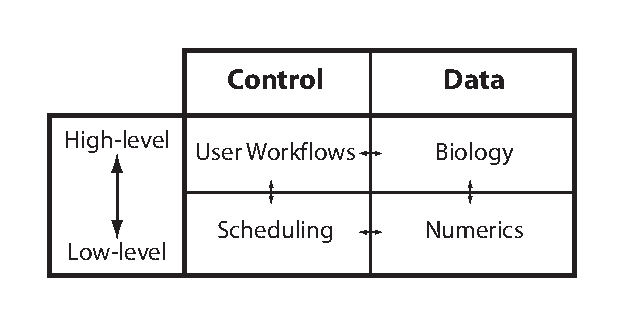
\includegraphics[scale=0.95]{figures/matrix.eps}
  %\caption{Relationships between data and control.}
  \label{fig:datacontrol}
\end{figure}

\subsubsection*{The requirement for data-layering}
\label{sec:data-layering}
The complex multi-dimensional nature of a biological system distinguishes it from the mathematical representations and data formats employed by a computer-based model of the system. Specifically, it is the dynamical properties of a biological system that do not map easily to the logical principles and mathematical constructs used by software implementations.

In the figure above, the horizontally directed arrows indicate the location of software control interfaces, whereas, the vertical arrows indicate the location of the data flow interfaces. It is notable that if software includes diagonal interfaces between blocks, e.g. between Biology and scheduling or User workflows and numerics, the result will will be an application that can be classed as monolithic. With these considerations in mind we have developed a software architecture meta-framework that has been used as a guide in the reconfiguration of GENESIS.

\subsection*{The Computational Biology Initiative Federated Software Architecture}

The CBI federated software architecture provides a modular paradigm that places stand-alone software components into logical relationships. It is referred to as being ``federated'' as it extends the modular approach  associated with the development of single applications to the functional integration of otherwise independent applications. In doing this the software architecture aims to provide a unified interface to diverse applications and mask from the user the differences, idiosyncracies, and implementations of the underlying applications and data sources.

The Data/Control schema illustrated above was developed into a software architecture giving the components that form the building blocks of the CBI architecture (illustrated in the following figure).  
\begin{figure}[h]
  \centering
 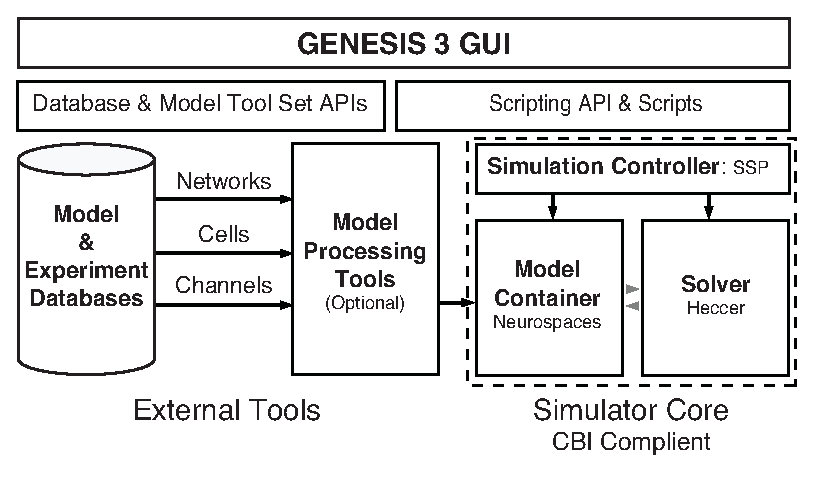
\includegraphics[scale=0.75]{figures/G3-Architecture-Overview-1.eps}
  %\caption{Overview of the Computational Biology Initiative Federated Software Architecture.}
  \label{fig:architecture1}
\end{figure}
Ideally, this architecture makes the underlying applications look to the user like a single system. This is achieved by recruiting different modules to provide the model building tools and simulator functionality required at the different stages of a project.

In summary, the CBI architecture provides a template for federated software development that, at its core, contains a CBI compliant simulator (the {\bf Model\,Container}, Simulation Controller ({\bf SSP}), Experimental Protocols ({\bf Experiment}) and Solver ({\bf Heccer}), located in the dashed box in the high level block diagram--above). It is the modularity of the architecture that simplifies connection to independent applications indirectly related to model construction and instantiation. In doing this it shares a number of ideas with the well-known three tier architectures paradigm (make link). The distinguishing feature of the CBI architecture is that the back-end comprises numerical solvers rather than relational databases.

The CBI compliant simulator indicated in the previous figure is expanded in the following figure to illustrate the key components. Data layers in the CBI architecture correspond to high-level data associated with biological concepts and extend to low level data such as numerical values employed by the solvers. The benefit of this layering of data is that it allows the mathematical and biological aspects of a model to be distinguished and separated by specific Data and Function bindings.

\begin{figure}[h]
  \centering
 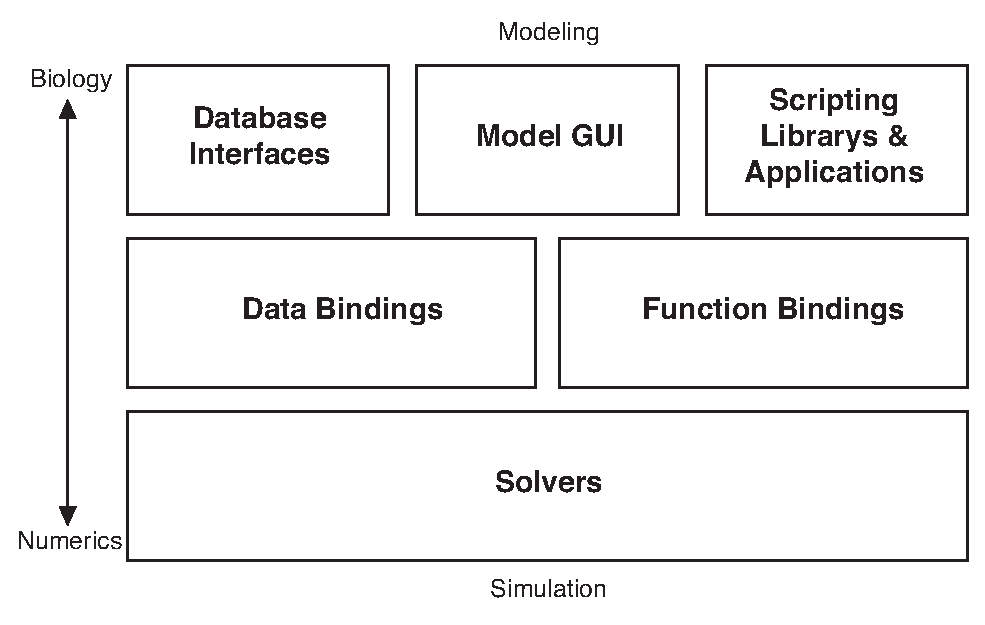
\includegraphics[scale=0.75]{figures/G3-CBI-Architecture-HiLevel.eps}
  %\caption{Key components of the simulator}
  \label{fig:archover}
\end{figure}

It is the clear delineation of the modules in the CBI architecture that allows both developers and users to choose to contribute to a single component with limited complexity, instead of being forced to contribute to the whole simulator and be exposed to tremendous complexity. Within the CBI paradigm each software component becomes self contained in the sense that it can be run independently. This has important advantages in that it facilitates the interoperability of software obtained from different sources by:

\begin{enumerate}
\item Reduced complexity of software modules compared to a unitary system.
\item Simplified documentation of modules in terms of inputs and outputs.
\item Easy incorporation or removal of individual modules as required.
\item Simplified development and testing of components as stand alone modules.
\item Clear delineation of scope for new module development.
\end{enumerate}

The CBI architecture provides three significant advantages for software development:

\begin{enumerate}
\item Modules can be run separately on different machines. For example, the GUI and modeling environment might run locally, while the simulator is run elsewhere either serially or in parallel on more powerful machines.
\item Decomposition of an application into multiple software components allows reuse and extension of individual modules, whether stand alone or otherwise, clearly facilitating model development and research progress.
\item Individual components can be independently updated, enhanced, or replaced when needed, thus the life cycle of a modular architecture is smoother than that of a non-scalable application.
\end{enumerate}

\subsection*{The GENESIS Project}

The recently developed CBI simulator architecture is an open framework that also provides a general context for ongoing GENESIS development. The architecture focuses users on the need to conceive, organize, execute and evaluate simulations, while allowing the development of new tools to support simulation based education, collaboration, and publication. The GENESIS modules that have been implemented, tested, and that are currently compliant with the CBI architecture include:

\begin{enumerate}
\item \href{../model-container/model-container.tex}{\bf Model\,Container:} Middle-ware dealing with biological entities and end-user concepts instead of mathematical equations. It is a declarative model container that generates highly efficient data structures implementing biological structures and components in a uniform data model across different levels of scale. When linked to a user interface it provides an efficient way to construct, inspect, and validate models.

\item \href{../experiment/experiment.tex}{\bf Experiment:} A library of experimental protocols such as voltage clamp and current clamp.

\item \href{../heccer/heccer.tex}{\bf Heccer:} A fast compartmental solver based on the GENESIS {\it hsolve} routine. The design flexibility of the architecture allows Heccer to be instantiated from from C, Perl, or other scripting languages.

\item {\href{../project-browser/project-browser.tex}{\bf Project\,Browser}:} A tool for inspection of projects and simulation results.

\item \href{../ssp/ssp.tex}{\bf Simple\,Scheduler\,in\,Perl:} {\bf SSP} builds simulation control files and can be constructed to bind the {\bf Model\,Container}, {\bf Experiment} and {\bf Heccer} and activate them correctly, such that they work together on a single simulation.

\item \href{../studio/studio.tex}{\bf Studio:} Provides tools for graphical browsing and command line usage.
\end{enumerate}

\subsection*{Planned External Interfaces for GENESIS}

Using the CBI architecture, GENESIS is being developed with the necessary interfaces that will, in principle, allow any simulation system to use its features. The figure below shows the multiple external interfaces to GENESIS that are planned for the new architecture.

\begin{figure}[h]
  \centering
 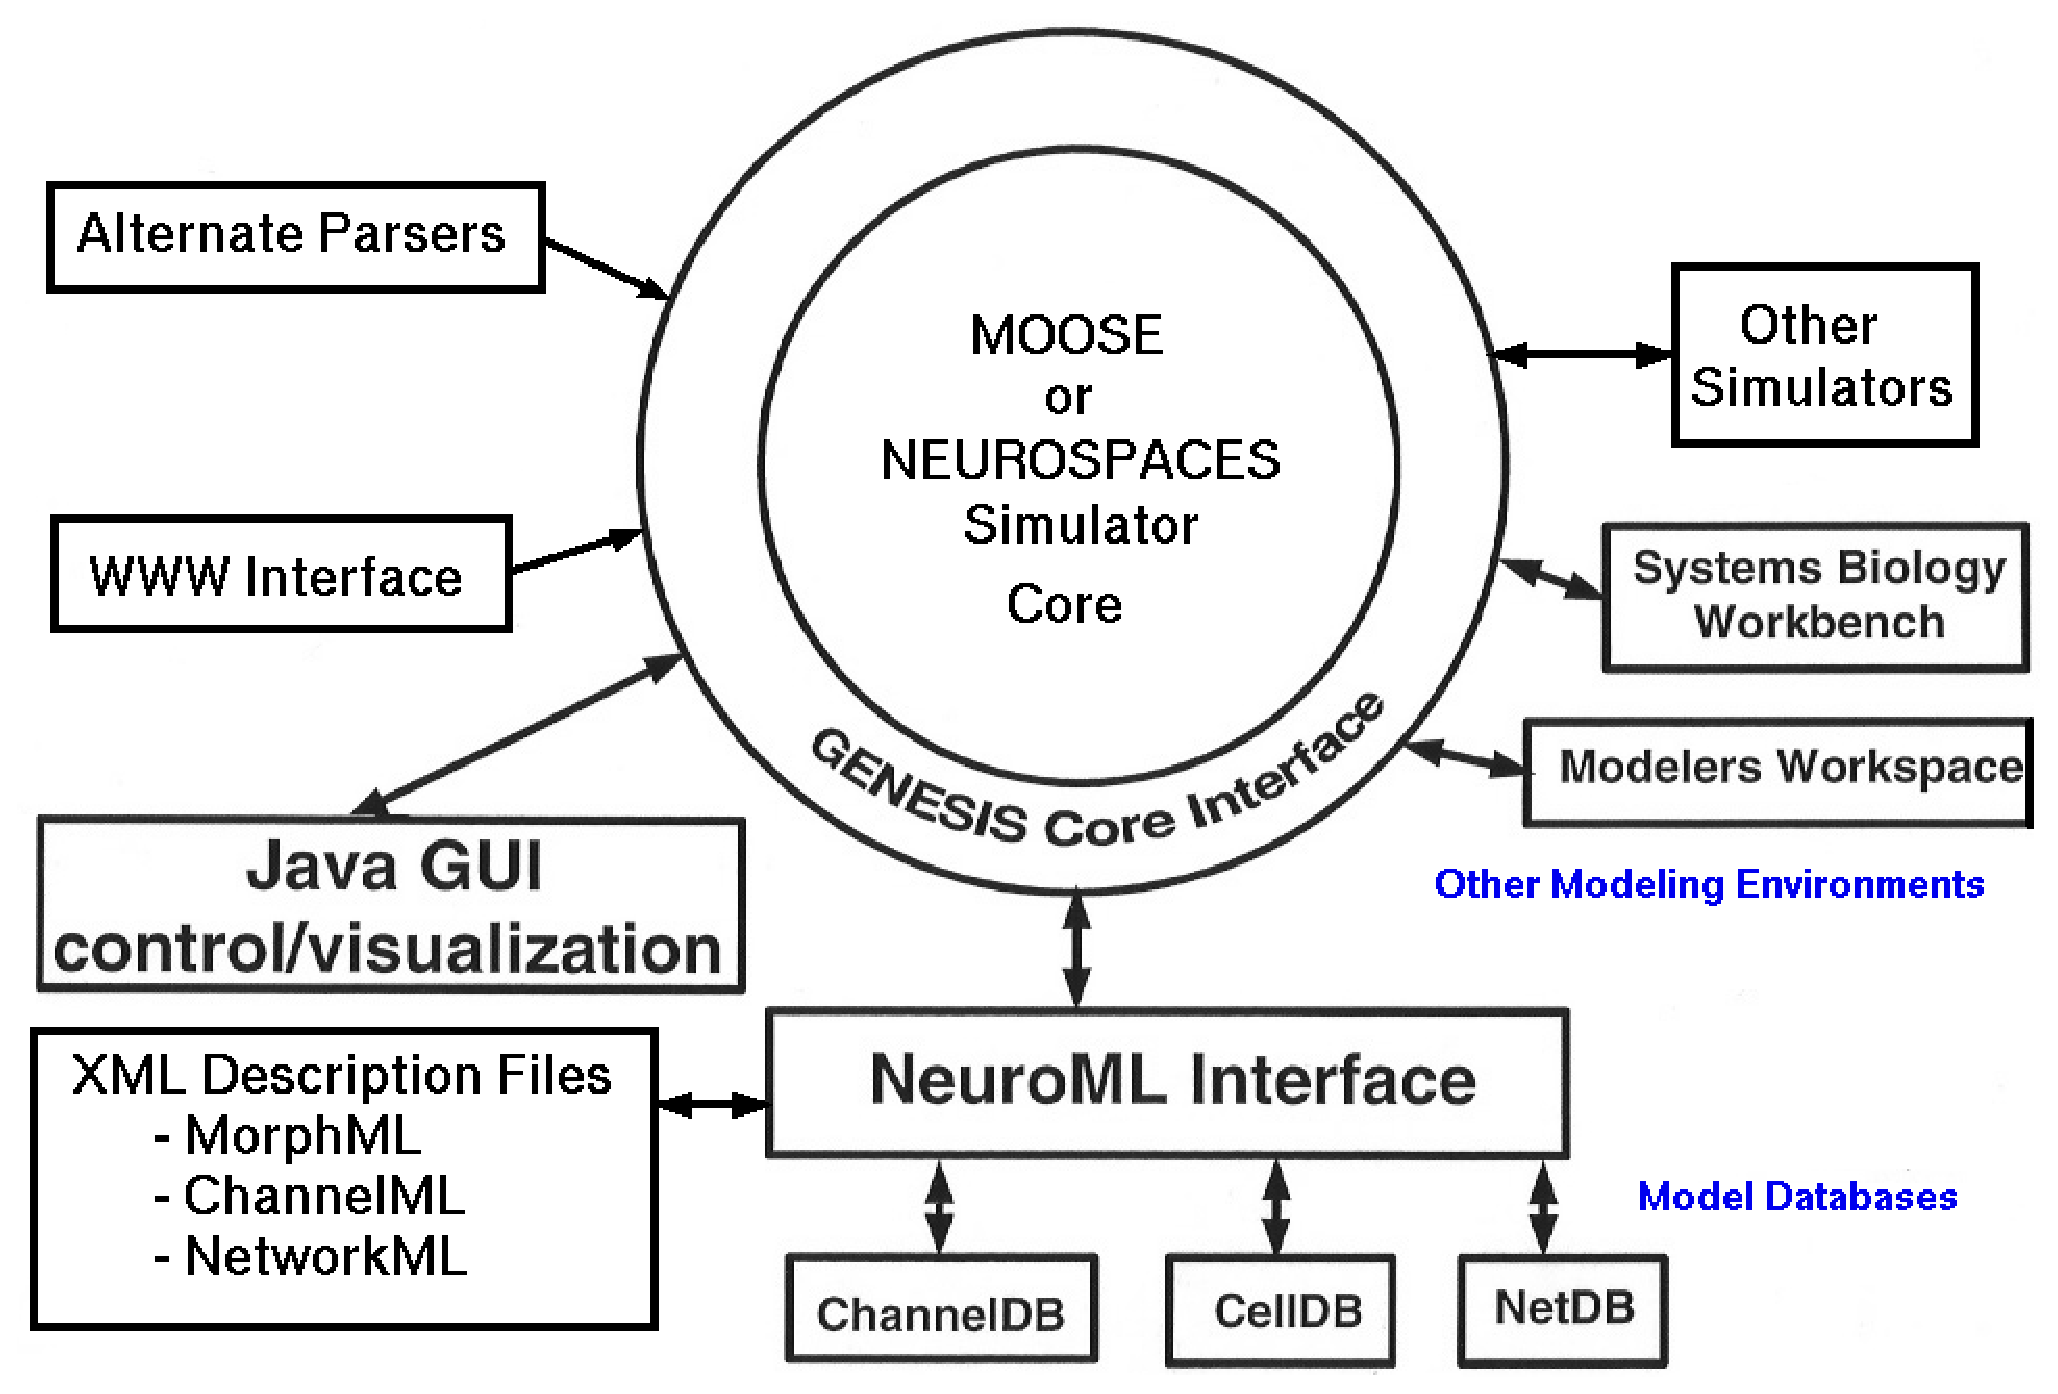
\includegraphics[scale=1.25]{figures/G3-Interfaces.eps}
  %\caption{enumerate}
  \label{fig:g3interfaces}
\end{figure}

\end{document}
